\section{48 - MAT - FA 2.2, AN 4.3, AN 1.3, AN 4.2 - Füllen eines Gefäßes - Matura 2014/15 Haupttermin}

\begin{langesbeispiel} \item[0] %PUNKTE DES BEISPIELS
				Der Innenraum eines 20 cm hohen Gefäßes hat in jeder Höhe $h$ eine rechteckige, horizontale Querschnittsfläche. Ihre Länge beträgt am Boden 10 cm und nimmt dann mit der Höhe linear bis auf 16 cm zu, ihre Breite beträgt in jeder Höhe 12 cm.
				
				\begin{center}
					\resizebox{0.6\linewidth}{!}{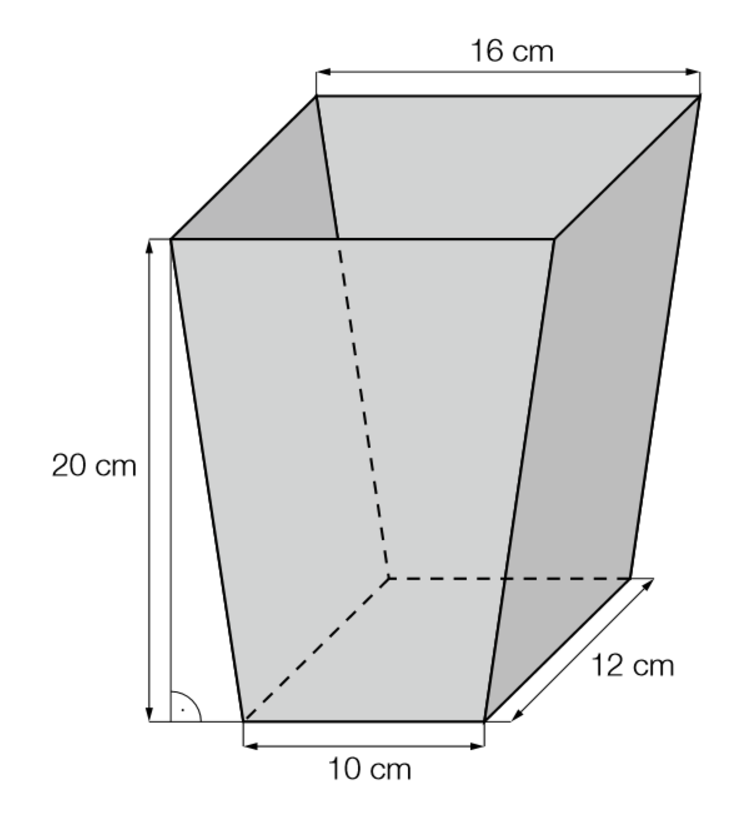
\includegraphics{../_database/Bilder/Bild48-1.eps}}
				\end{center}


\subsection{Aufgabenstellung:}
\begin{enumerate}
	\item \fbox{A} Gib eine Formel für die Länge $a(h)$ der rechteckigen Querschnittsfläche in der Höhe $h$ an.
	
	In das Gefäß wird Flüssigkeit gefüllt.
	
	Gib an, was der Ausdruck $12\cdot\displaystyle\int^{15}_0{a(h)}$d$h$ in diesem Zusammenhang bedeutet!
\item Das leere Gefäß wird bis zum Rand mit Flüssigkeit gefüllt.

Nach $t$ Sekunden befindet sich die Wassermenge $q(t)$ (in ml) im Gefäß. Die Füllung dauert 39 Sekunden. Für $t\in[0;39]$ gilt: $q'(t)=80$.

Interpretiere $q'(t)=80$ im gegebenen Zusammenhang!

Ermittle $\frac{q(t_2)-q(t_1)}{t_2-t_1}$ für beliebige $t_1,t_2$ mit $t_1<t_2$ aus dem gegebenen Zeitintervall!
\item Das Fassungsvermögen des Gefäßes (in ml) bis zur Höhe $x$ kann durch das Integral $\int^x_0{(3,6\cdot h+120)}$d$h$ dargestellt werden.

Ermittle, bei welcher Höhe $x$ das Wasser im Gefäß steht, wenn man 2,5 Liter Wasser in das Gefäß gießt.

Interpretiere den im Integral vorkommenden Wert $3,6$ im gegebenen Kontext!
						\end{enumerate}\leer
				
\antwort{
\begin{enumerate}
	\item \subsection{Lösungserwartung:} 
	
	$a(h)=k\cdot h+d$
	
	$a(0)=d=10$
	
	$a(20)=20\cdot k+10=16 \Rightarrow k=0,3$
	
	$a(h)=0,3\cdot h+10$
	
	Das Integral gibt das Volumen der enthaltenen Flüssigkeit (in ml) an, wenn das Gefäß bis 5 cm unter dem Rand (bzw. bis zu einer Höhe von 15 cm) gefüllt ist.	 	
	\subsection{Lösungsschlüssel:}
	\begin{itemize}
		\item  Ein Ausgleichspunkt für eine korrekte Formel. Äquivalente Formeln sind ebenfalls als richtig zu werten. Die Aufgabe ist auch dann als richtig gelöst zu werten, wenn bei korrektem Ansatz das Ergebnis aufgrund eines Rechenfehlers nicht richtig ist.
		\item  Ein Punkt für eine (sinngemäß) korrekte Interpretation.
	\end{itemize}
	
	\item \subsection{Lösungserwartung:}
			
		Die momentane Änderungsrate der Wassermenge beträgt im gesamten Zeitintervall 80 Milliliter pro Sekunde.
		
		$\dfrac{q(t_2)-q(t_1)}{t_2-t_1}=80$

	\subsection{Lösungsschlüssel:}
	
\begin{itemize}
	\item Ein Punkt für eine (sinngemäß) korrekte Interpretation.
	\item Ein Punkt für die richtige Lösung.
\end{itemize}

\item \subsection{Lösungserwartung:}
	$2500=\int^x_0{(3,6\cdot h+120)}$d$h=1,8x^2+120x$
	
	$1,8x^2+120x-2500=0$
	
	$x_1\approx 16,7, (x_2<0)$
	
	Das Wasser steht ca. 16,7 cm hoch.
	
	3,6 gibt diejenige Fläche in cm$^2$ an, um die die Querschnittsfläche mit jedem zusätzlichen cm Höhe zunimmt. 
	
	oder: 
	
	3,6 ist die Steigung der Funktion, die den Inhalt der Querschnittsfläche in der Höhe $h$ angibt.

	\subsection{Lösungsschlüssel:}
	
\begin{itemize}
	\item Ein Punkt für die richtige Lösung, wobei weder die negative Lösung der quadratischen Gleichung noch die Einheit cm angeführt werden müssen.
		
		Toleranzintervall: $[16,5; 17]$  
		
		Die Aufgabe ist auch dann als richtig gelöst zu werten, wenn bei korrektem Ansatz das Ergebnis aufgrund eines Rechenfehlers nicht richtig ist. 
	\item Ein Punkt für eine (sinngemäß) korrekte Interpretation.
\end{itemize}

\end{enumerate}}
		\end{langesbeispiel}